\documentclass[12pt,a4paper]{article}
\usepackage[utf8]{inputenc}
\usepackage{amsmath}
\usepackage{amsfonts}
\usepackage{amssymb}

%bold Greek letters and other symbols
\usepackage{bm}
\usepackage{graphics}
\usepackage[T1]{fontenc}
\usepackage[english]{babel}
\usepackage{graphicx}
\usepackage[left=2.5cm,right=3.0cm,top=2.5cm,bottom=3cm]{geometry}
\usepackage{color}
%
\usepackage{makeidx}
\usepackage{shortvrb,latexsym}

\setlength{\parindent}{0pt}
%\renewcommand{\floatpagefraction}{.99}
%\renewcommand{\textfraction}{.01}
\def \uu  {\bm{u}}
\def \oo {\bm{\omega}}
\def \curl {\bm{\nabla}\times}
\def \dive {\bm{\nabla}\cdot}
\def \AA  {\bm{A}}
\newcommand{\bu}{\bm{u}}
\newcommand{\bv}{\bm{v}}
\newcommand{\br}{\bm{r}}
\newcommand{\rd}{\mathrm{d}}
\newcommand{\hx}{{\bf\hat{x}}}
\newcommand{\hy}{{\bf\hat{y}}}
\newcommand{\hz}{{\bf\hat{z}}}
\newcommand{\hr}{{\bf\hat{r}}}
\newcommand{\hn}{{\bf\hat{n}}}

\begin{document}

\begin{center}
2023-08-24
\end{center}
STOCKHOLMS UNIVERSITET\\
Meteorologiska Institutionen\\
Jonas Nycander, Dhrubaditra Mitra\\
\vspace{1cm}

\begin{center}
{\bf\large Exam in Fluid mechanics (MO5001)}\\
\end{center}

Write the solution of each problem on a separate paper, and write your identification number on every paper.\\

{\bf Allowed aids:} calculator, sheet with vector analysis relations.\\

{\bf Grading:} A 90-100\%, B 80-89\%, C 65-79\%, D 55-64\%, E 50-54\%, Fx 45-49\%, F 0-44\% \\
\vspace{0.5cm}

\begin{enumerate}

\item \label{prb1}

  While cooking last night, I put my chopping board on the
    kitchen counter. I had not noticed that there was a small amount
    of water on the kitchen counter already. After using the board I
    tried to lift it up in the way I sketch in
    figure~\ref{fig:board}. I realised that I had to exert a force much
    larger than the weight of the board itself.
  \begin{figure}[h]
    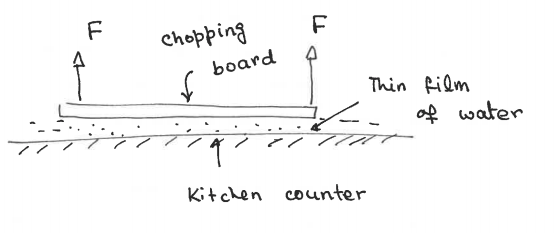
\includegraphics[width=0.5\linewidth]{board.png}
    \label{fig:board}
   \end{figure}
    \begin{enumerate}
    \item Explain qualitatively (and concisely) why ? (3 p)
    \item Assume that the shape of my chopping board is a circular
      disk of radius $a$. The thickness of the film of
      water trapped between the board and the kitchen counter is $h$.
      Calculate the force necessary to pull the board by a distance
      $\Delta h$ in time $\Delta t$. State clearly all the assumption
      you need to make to solve this problem. (7 p)
    \end{enumerate}
%---------------------------------------------------------%
\item
  \label{prb2} A thin rectangular plate of dimension $L_x\times L_z$ 
is immersed in a fluid  of
kinematic viscosity $\nu$ and density $\rho$. The plate is being
pulled by a force such that it moves with a velocity $v$ along the $x$
direction. Far away from the plate the fluid is at rest. Assume that the flow is
  laminar. Ignore the edge effects. 
  Estimate the the power necessary to keep the plate moving with a constant velocity.
    (Hint : The power necessary
    is equal to the power dissipated by the viscous forces. You can estimate the
    viscous forces from the stress at the surface of the disc. You need the
    thickness of the boundary layer to estimate the stress. ) (5p)
 
%---------------------------------------------------------%
\item
\label{prb3}
Answer the following short questions. You just need to write the final answer.
Each question is worth 2 points. 
  \begin{enumerate}
  \item A scalar function of three Cartesian coordinates, $x,y,z$ is 
    \begin{equation}
       T(x,y,z) = \sin(x)\cos(y) + \cos(y)\sin(z)
    \end{equation}
    If $\vec{G} = \vec{\nabla} T $ then calculate $\vec{\nabla}\times \vec{G}$.
  \item After deformation the displacement field in a material is given by the
    following expression
    \begin{eqnarray}
      u_x = \alpha [2x + \sin(y) + 5z^3 ] \\
      u_y = \alpha[ e^{-x} - y + \cos(z) ] \\
      u_z = \alpha[ \sin(x) + \cos(y) -z ]
    \end{eqnarray}
    Here $\alpha$ is small such that you can apply the approximation of small deformation
    everywhere. Under this deformation calculate the change is volume of the material.
  \item In which of the following cases can I write the velocity $\vec{v} = \nabla \Psi $ where $\Psi$ is a scalar function
    without any loss of generality: \\
    (a) if the flow is incompressible, (b) if the flow is irrotational, or (c) if the flow is steady.
  \item In a turbulent boundary layer very close to the wall how does the mean stream-wise
    velocity ($\langle v_x \rangle$) depends on the wall-normal coordinate ($y$) ? 
 \item Which of the following are true ? (More than one may be true. )
   Viscosity of a Newtonian fluid is
   \begin{enumerate}
   \item a scalar.
   \item can be described by two scalar quantities.
     \item is a fourth rank tensor. 
    \end{enumerate}
\end{enumerate}


(10 p)
%---------------------------------------------------------%
\item
The horizontal component of the Navier-Stokes equations in a rotating
system is
$$
\frac{\partial\bu}{\partial t}+\bu\cdot\nabla\bu+f\hz\times\bu =
-\frac{\nabla p}{\rho}+\nu\nabla^2 \bu,
$$
where the velocity $\bu$ is assumed to be purely horizontal.
\begin{enumerate}
  \item Define the Rossby number and the Ekman number in terms of the time
  scale $T$, horizontal length scale $L$ and vertical length scale $H$,
  and explain how these numbers measure the ratio between various
  terms in the equation above. Also give the thickness of the Ekman layer.
  \item Simplify the equation above for the case that $\bu$ is stationary
  and horizontally homogeneous, i.e.\ does not depend on $t, x$ or $y$.
  \item A constant wind blows over the ocean and exerts the wind stress
  $\bm{\tau}$ on the surface of the ocean. Give the appropriate
  boundary condition for the flow $\bu$ in the ocean.
  \item Assume that there is no geostrophic flow, and determine the volume
  flux in the ocean Ekman layer.
\end{enumerate}

(10 p)\\
%---------------------------------------------------------%
\item
The rotating shallow-water equations are
$$
\frac{\partial \bu}{\partial t}+\bu\cdot\nabla\bu+f\hz\times\bu
= -g\nabla h,
$$
$$
\frac{\partial h}{\partial t}+\nabla\cdot(\bu h) = 0,
$$
where $h$ is the  depth and $\bu$ the velocity.
\begin{enumerate}
\item Mention two different kinds of waves that can be described by these equations. 
\item The equations can describe a slow mode and a fast mode. What assumption
must be made to derive an equation that only describes the slow mode? Motivate the answer.
\item The potential vorticity for the shallow-water equations is defined by
$$
q = \frac{f(y)+\zeta}{h},
$$
where $\zeta=\partial v/\partial x-\partial u/\partial y$ is the relative vorticity. Describe the
conservation law for potential vorticity in words, and write it as an equation.
\end{enumerate}

(5 p)\\
%---------------------------------------------------------%
\item An ocean current flows northeastward at the latitude 20$^\circ$N. The current is 
barotropic, i.e.\ the velocity is uniform from the bottom to the surface, and the local
depth of the ocean is 3000 m. The Rossby number of the flow is very small, much smaller than 0.1.
\begin{enumerate}
 \item When the current reaches the latitude 30$^\circ$N the Rossby number is still very small.
 What is the local depth of the ocean?
 \item Suppose that the current instead flowed along contours of constant depth.
 What would the Rossby number and the relative vorticity be when it reached 30$^\circ$N?
\end{enumerate}

(5 p)\\
%---------------------------------------------------------%
\item
A fluid layer  is bounded by vertical walls at $x = 0$ and $x = L$. The bottom is flat, and the 
layer thickness is $h_{0}$ at $x = 0$ and $h_{L}$ at $x = L$. Calculate the northward 
volume transport between the walls. Assume that the flow is governed by the rotating 
shallow-water equations:
$$  
\frac{\partial \bu}{\partial t}+\bu\cdot\nabla\bu+f\hz\times\bu
= -g\nabla h,
$$
$$
\frac{\partial h}{\partial t}+\nabla\cdot(\bu h) = 0,
$$
where $h$ is the depth and $\bu$ the velocity. The flow is steady, and $\bu = v(x)\hy$.
  
(5 p)\\
%---------------------------------------------------------%

\end{enumerate}

\end{document}
